\subsection{Filtered Poisson process}

\begin{frame}{Filtered Poisson process --- Examples}

    The FPP model intermittent processes:\vspace{-13mm}
    \begin{figure}
        \centering
        \visible<2->{
            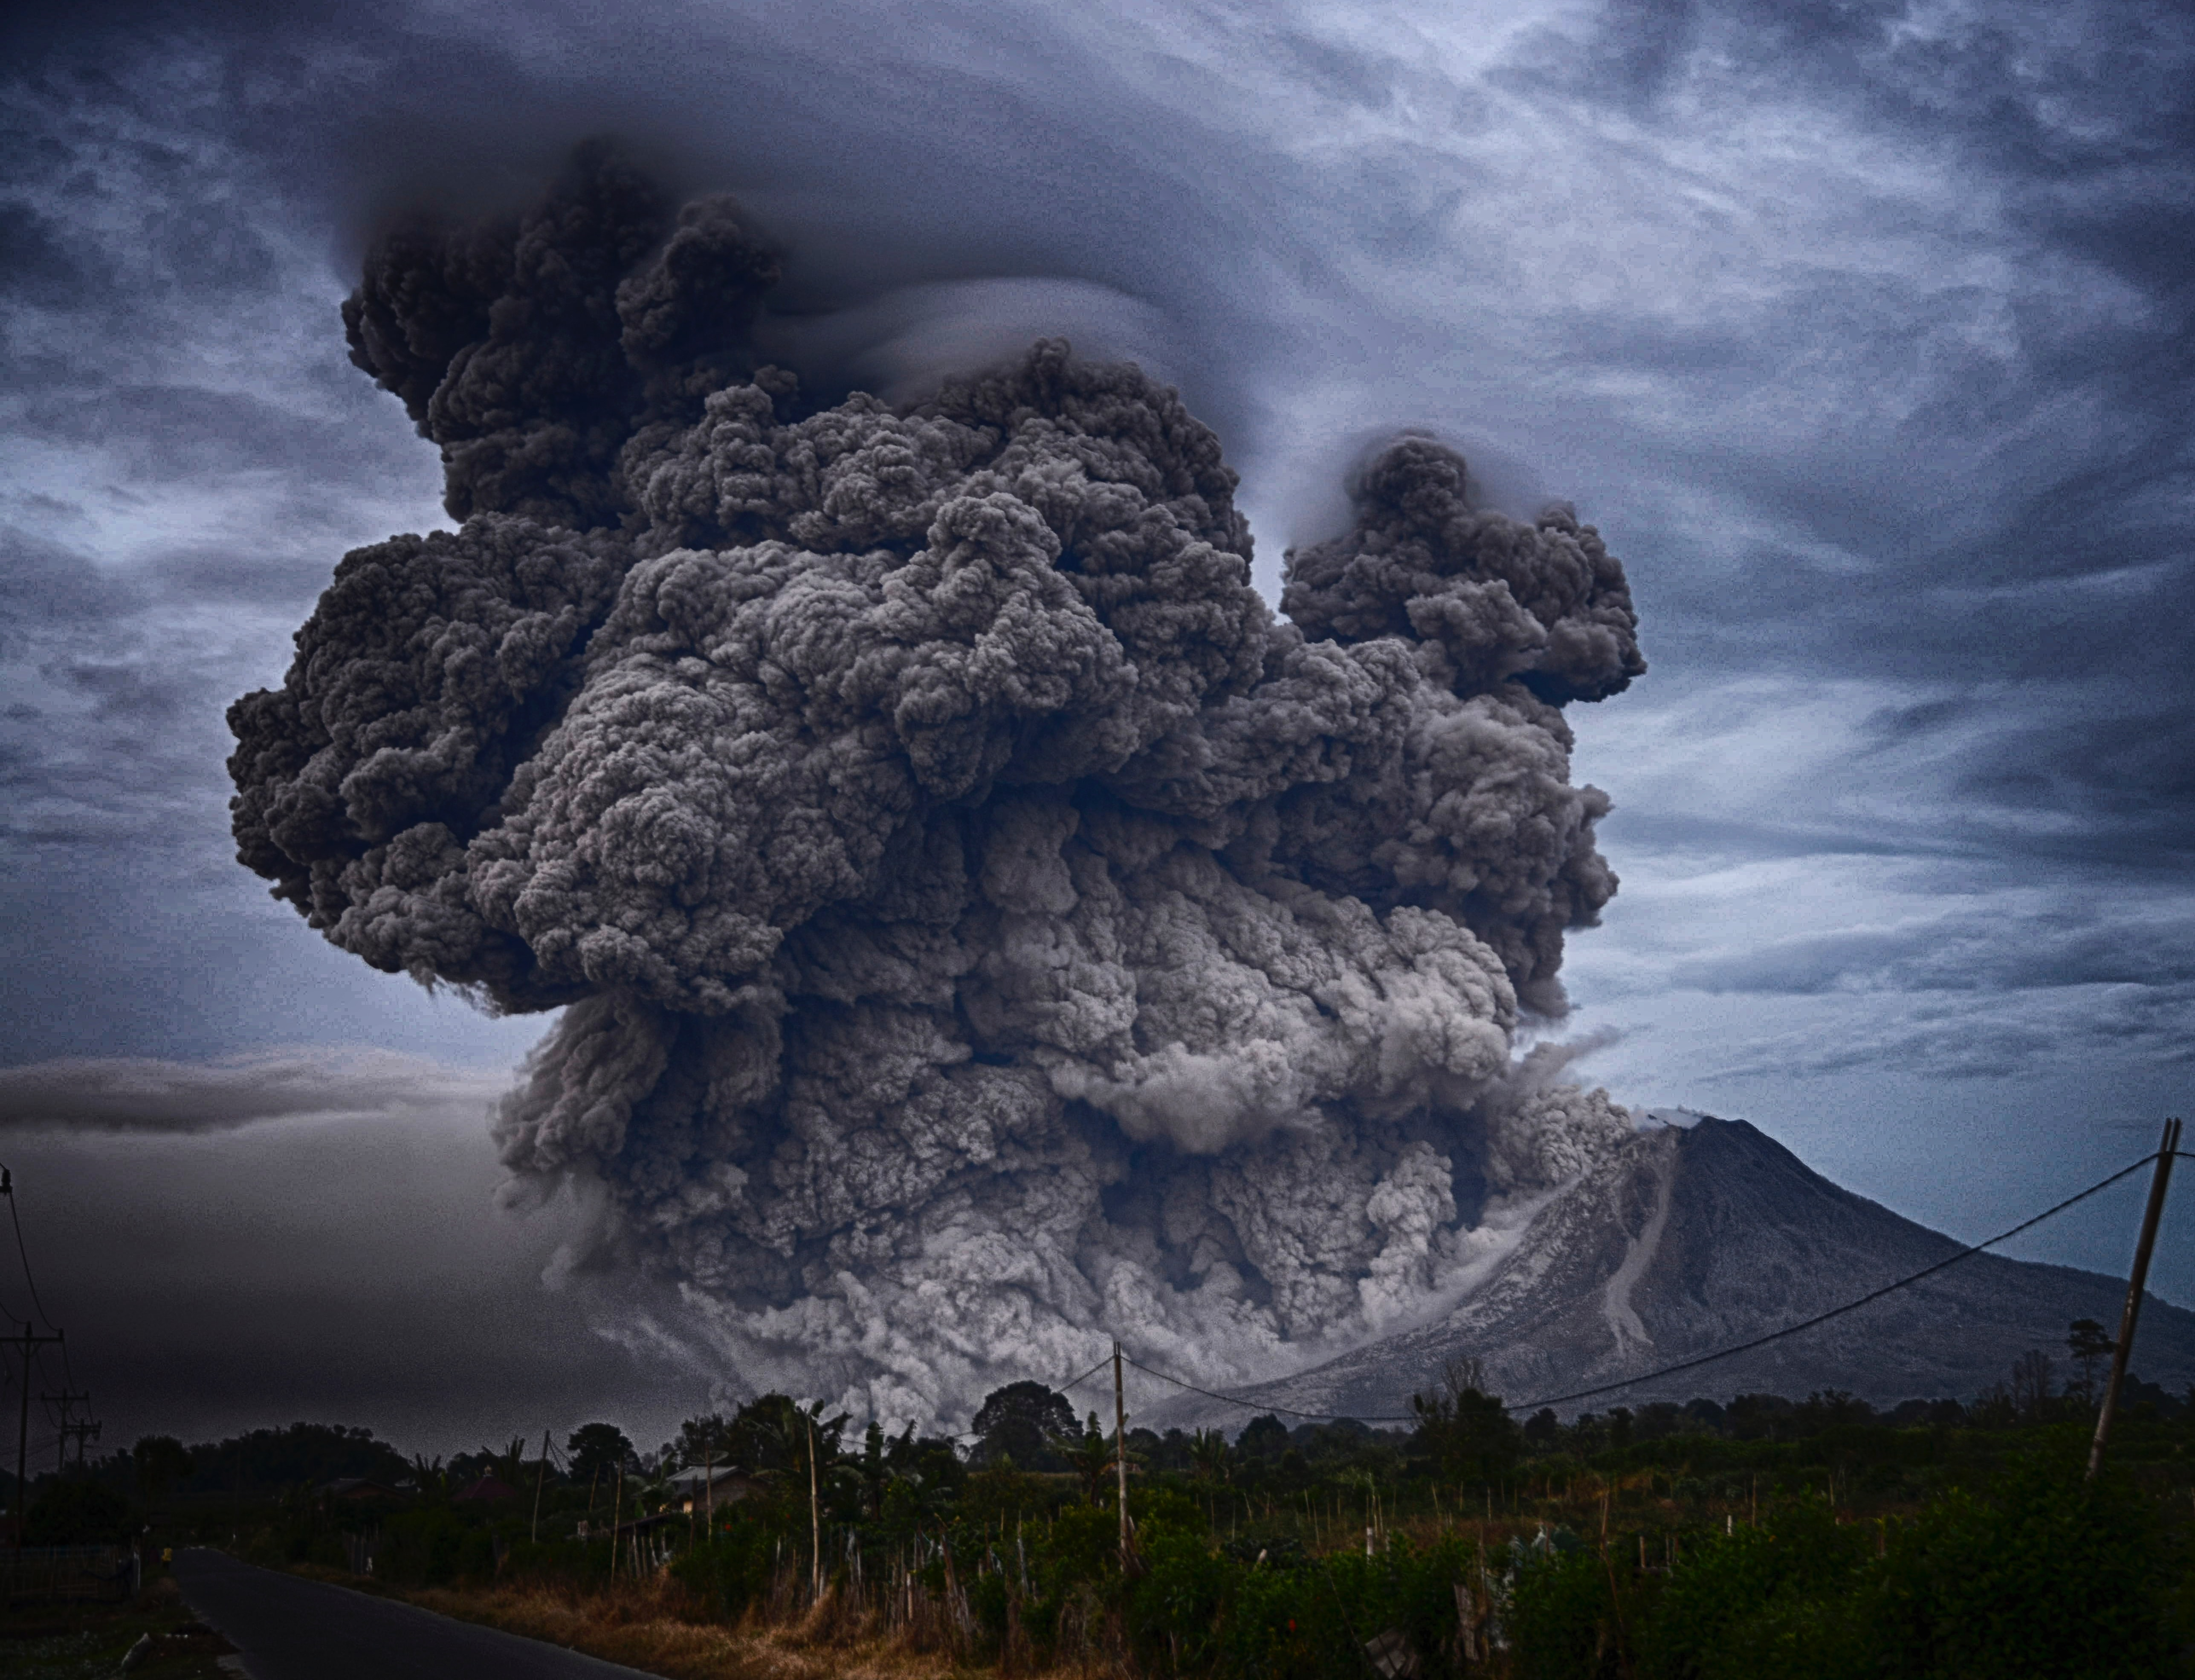
\includegraphics[width=.31\linewidth]{unsplash/volcano-unsplash.jpg}
        }
        \visible<3->{
            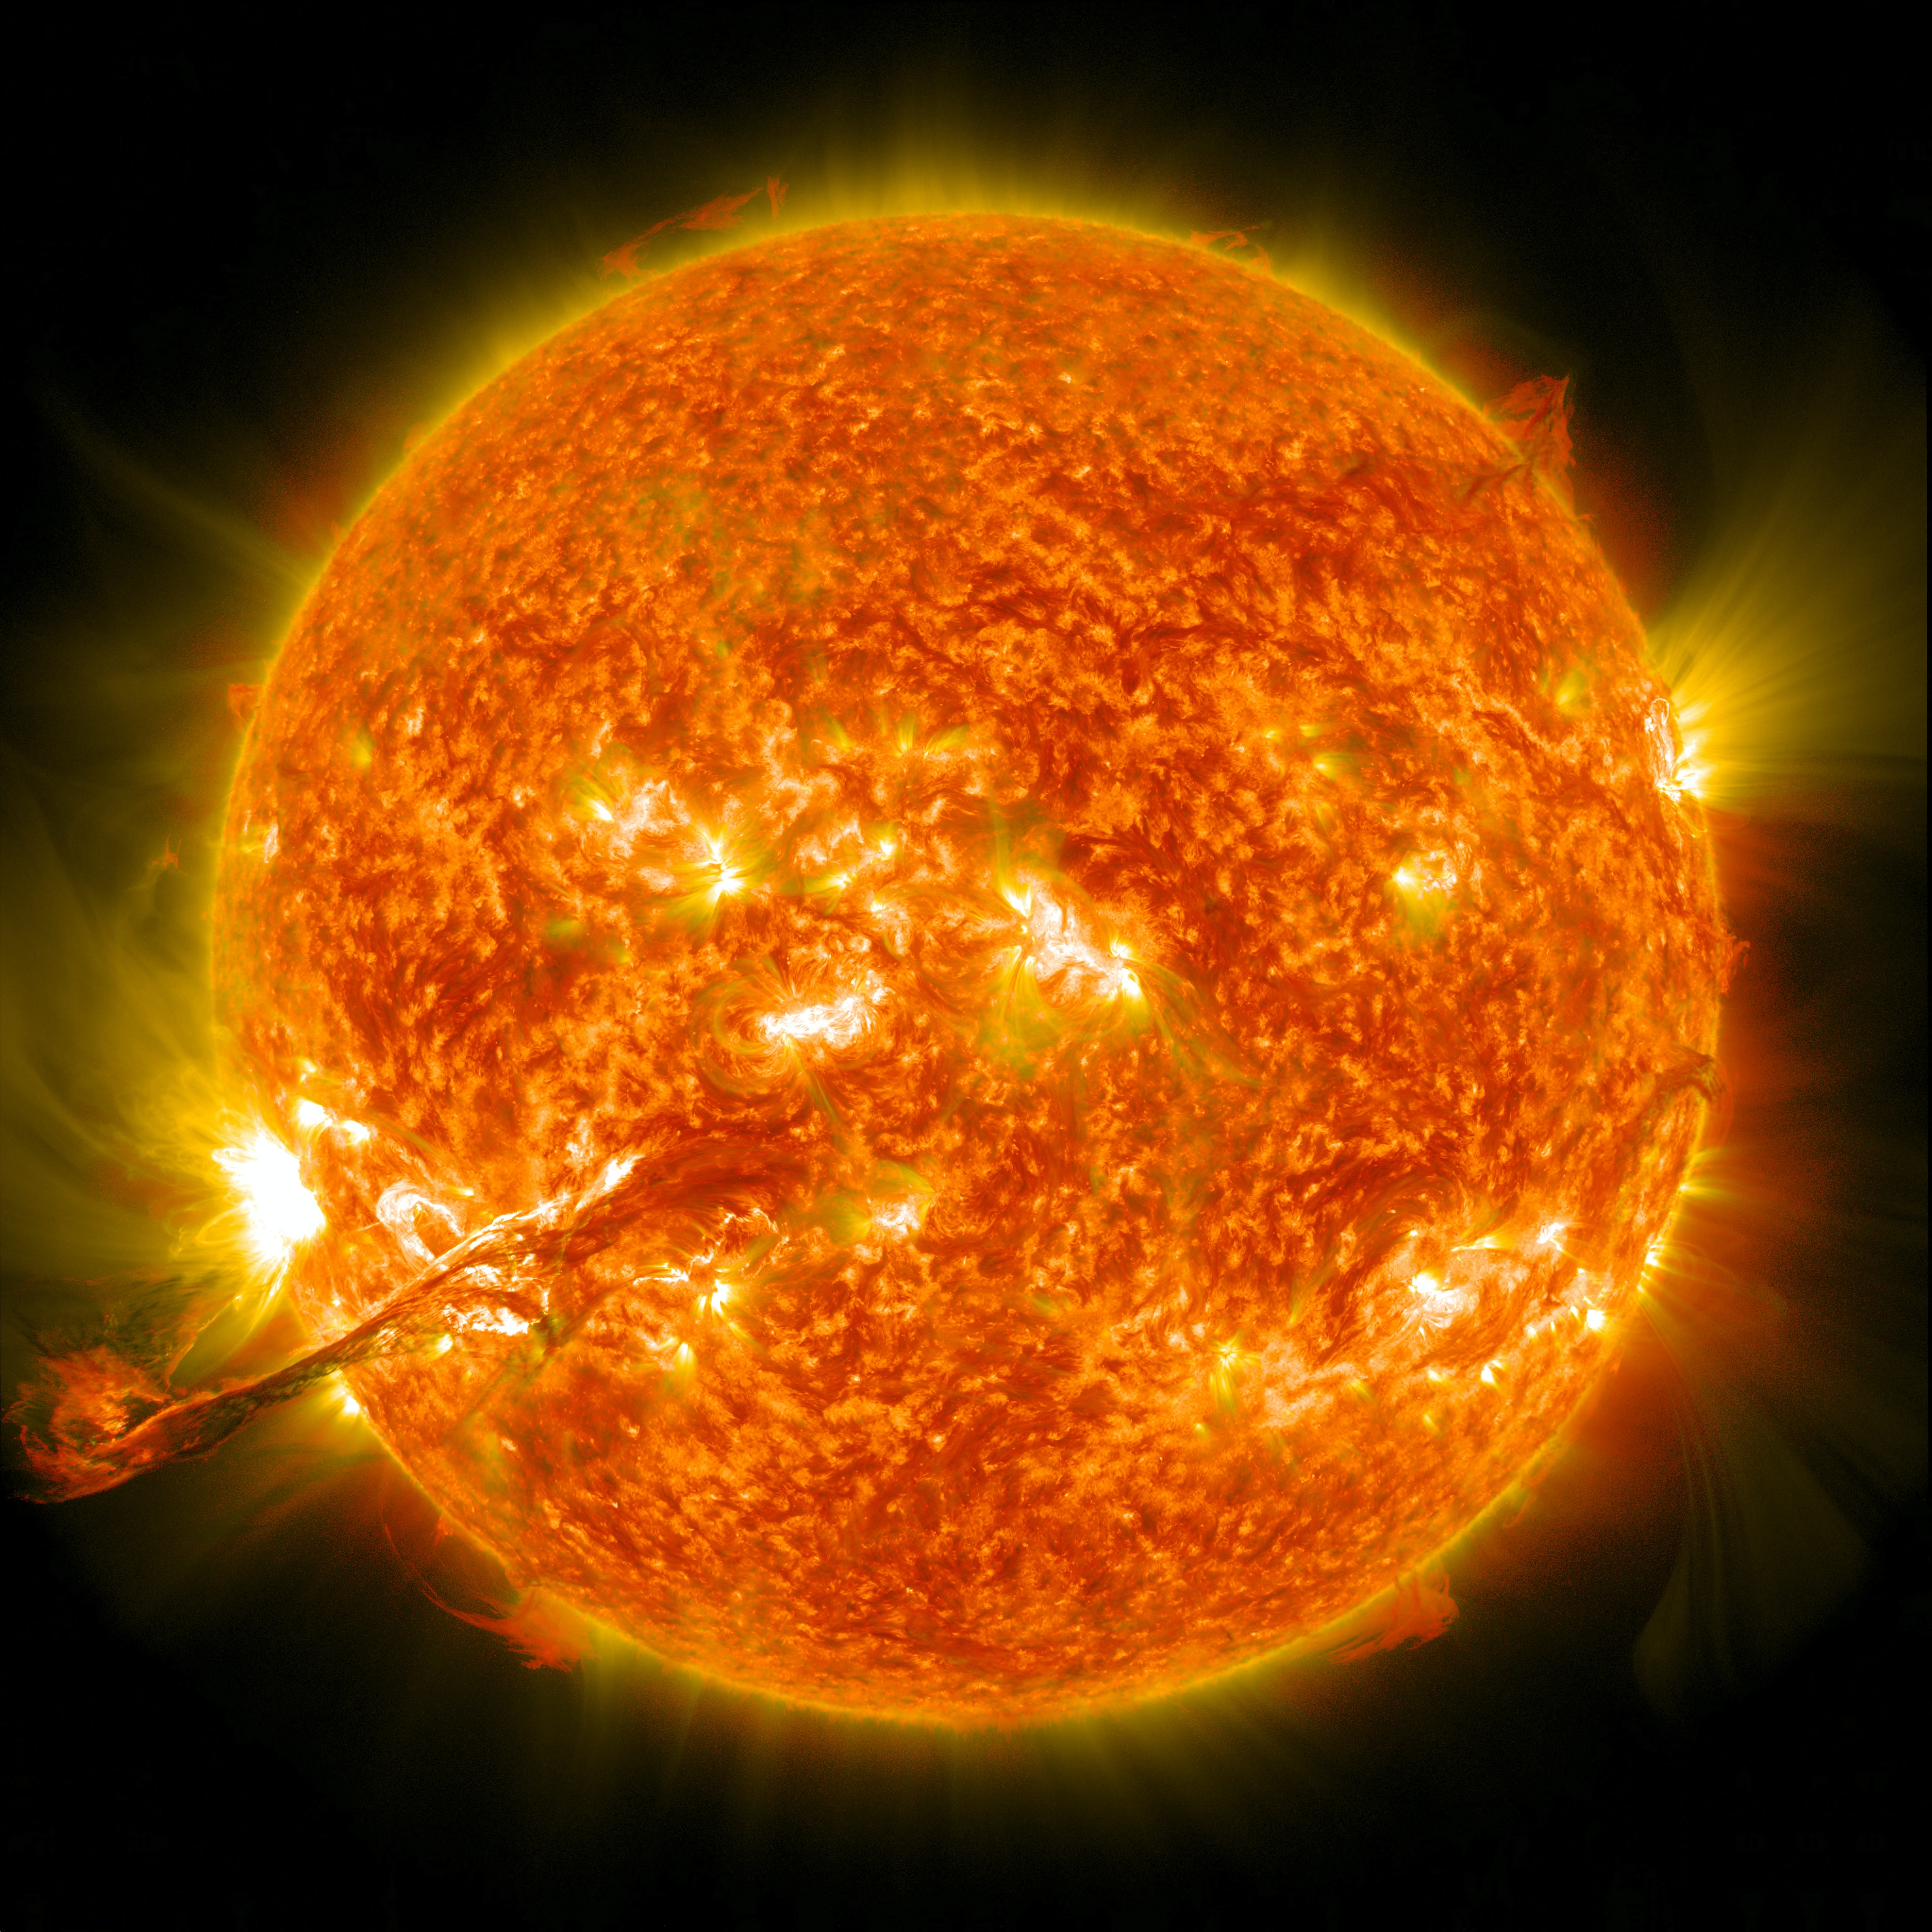
\includegraphics[width=.31\linewidth]{unsplash/nasa-cme-unsplash.jpg}%
        }%
        \visible<4>{
            % \copyrightbox[r]{
            %     % \includemovie{1cm}{1cm}{nstx/nstx.gif}
            %     \movie[
            %     height=.45\linewidth,
            %     width=.3\linewidth,
            %     autostart,
            %     loop
            %     ]{}{nstx/nstx.gif}
            % }
            % {\tiny\textbf{NSTX GPI Library} (2010 data)}
            \copyrightbox[r]{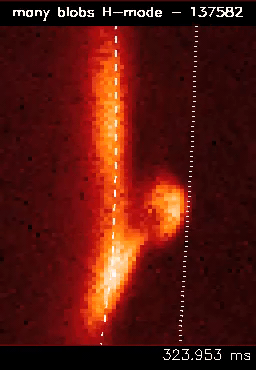
\includegraphics[width=.31\linewidth]{blobs/blobpng_284.png}}
            {\tiny\textbf{NSTX GPI Library} (2010 data)}
        }
    \end{figure}

    \note<+>{
        \begin{itemize}
            \item As our model we use the filtered Poisson process, which is a
                phenemenological model describing intermittent processes
            \item This means the model does not in itself give any insight in some
                specific physical process, but it is a powerful tool that can be used
                to investigate phenomena that show intermittency
        \end{itemize}
    }
    \note<+>{
        \begin{itemize}
            \item One example is temperature response to volcanoes which we will look at in this presentation
        \end{itemize}
    }
    \note<+>{
        \begin{itemize}
            \item Such processes can also be found in solar flares
        \end{itemize}
    }
    \note<+>{
        \begin{itemize}
            \item Or as Sajidah showed in her talk, fluctuations in fusion plasma devices
        \end{itemize}
    }

\end{frame}

\begin{frame}{Filtered Poisson process --- Definition}

    The underlying phenemenological model:

    \begin{columns}
        \begin{column}{.51\linewidth}
            \begin{equation}\label{eq:fpp_sum}
                % \alt<2>{T_K(t)}{\Phi_K(t)}=\sum_{k=1}^{\alt<2>{K}{K(T)}} A_k \phi\left(\frac{t-t_k}{\tau_\mathrm{d}}\right)
                T_K(t)=\sum_{k=1}^{K} \alt<2>{\alert{A_k}}{A_k} \phi
                \left(\frac{t-\alt<3>{\alert{t_k}}{t_k}}{\alt<4>{\alert{\tau_\mathrm{d}}}{\tau_\mathrm{d}}}\right)
            \end{equation}
            \visible<5->{\vspace{-3mm}
                \begin{equation*}
                    \downarrow
                \end{equation*}
                \begin{equation}\label{eq:fpp_convolve}
                    % \alt<2>{T_K(t)}{\Phi_K(t)}=[\phi * f_K]\left(\frac{t}{\tau_\mathrm{d}}\right)
                    T_K(t)=[\phi * f_K]\left(\frac{t}{\tau_\mathrm{d}}\right)
                \end{equation}
            }
        \end{column}
        \begin{column}{.65\linewidth}
            \begin{figure}
                \centering
                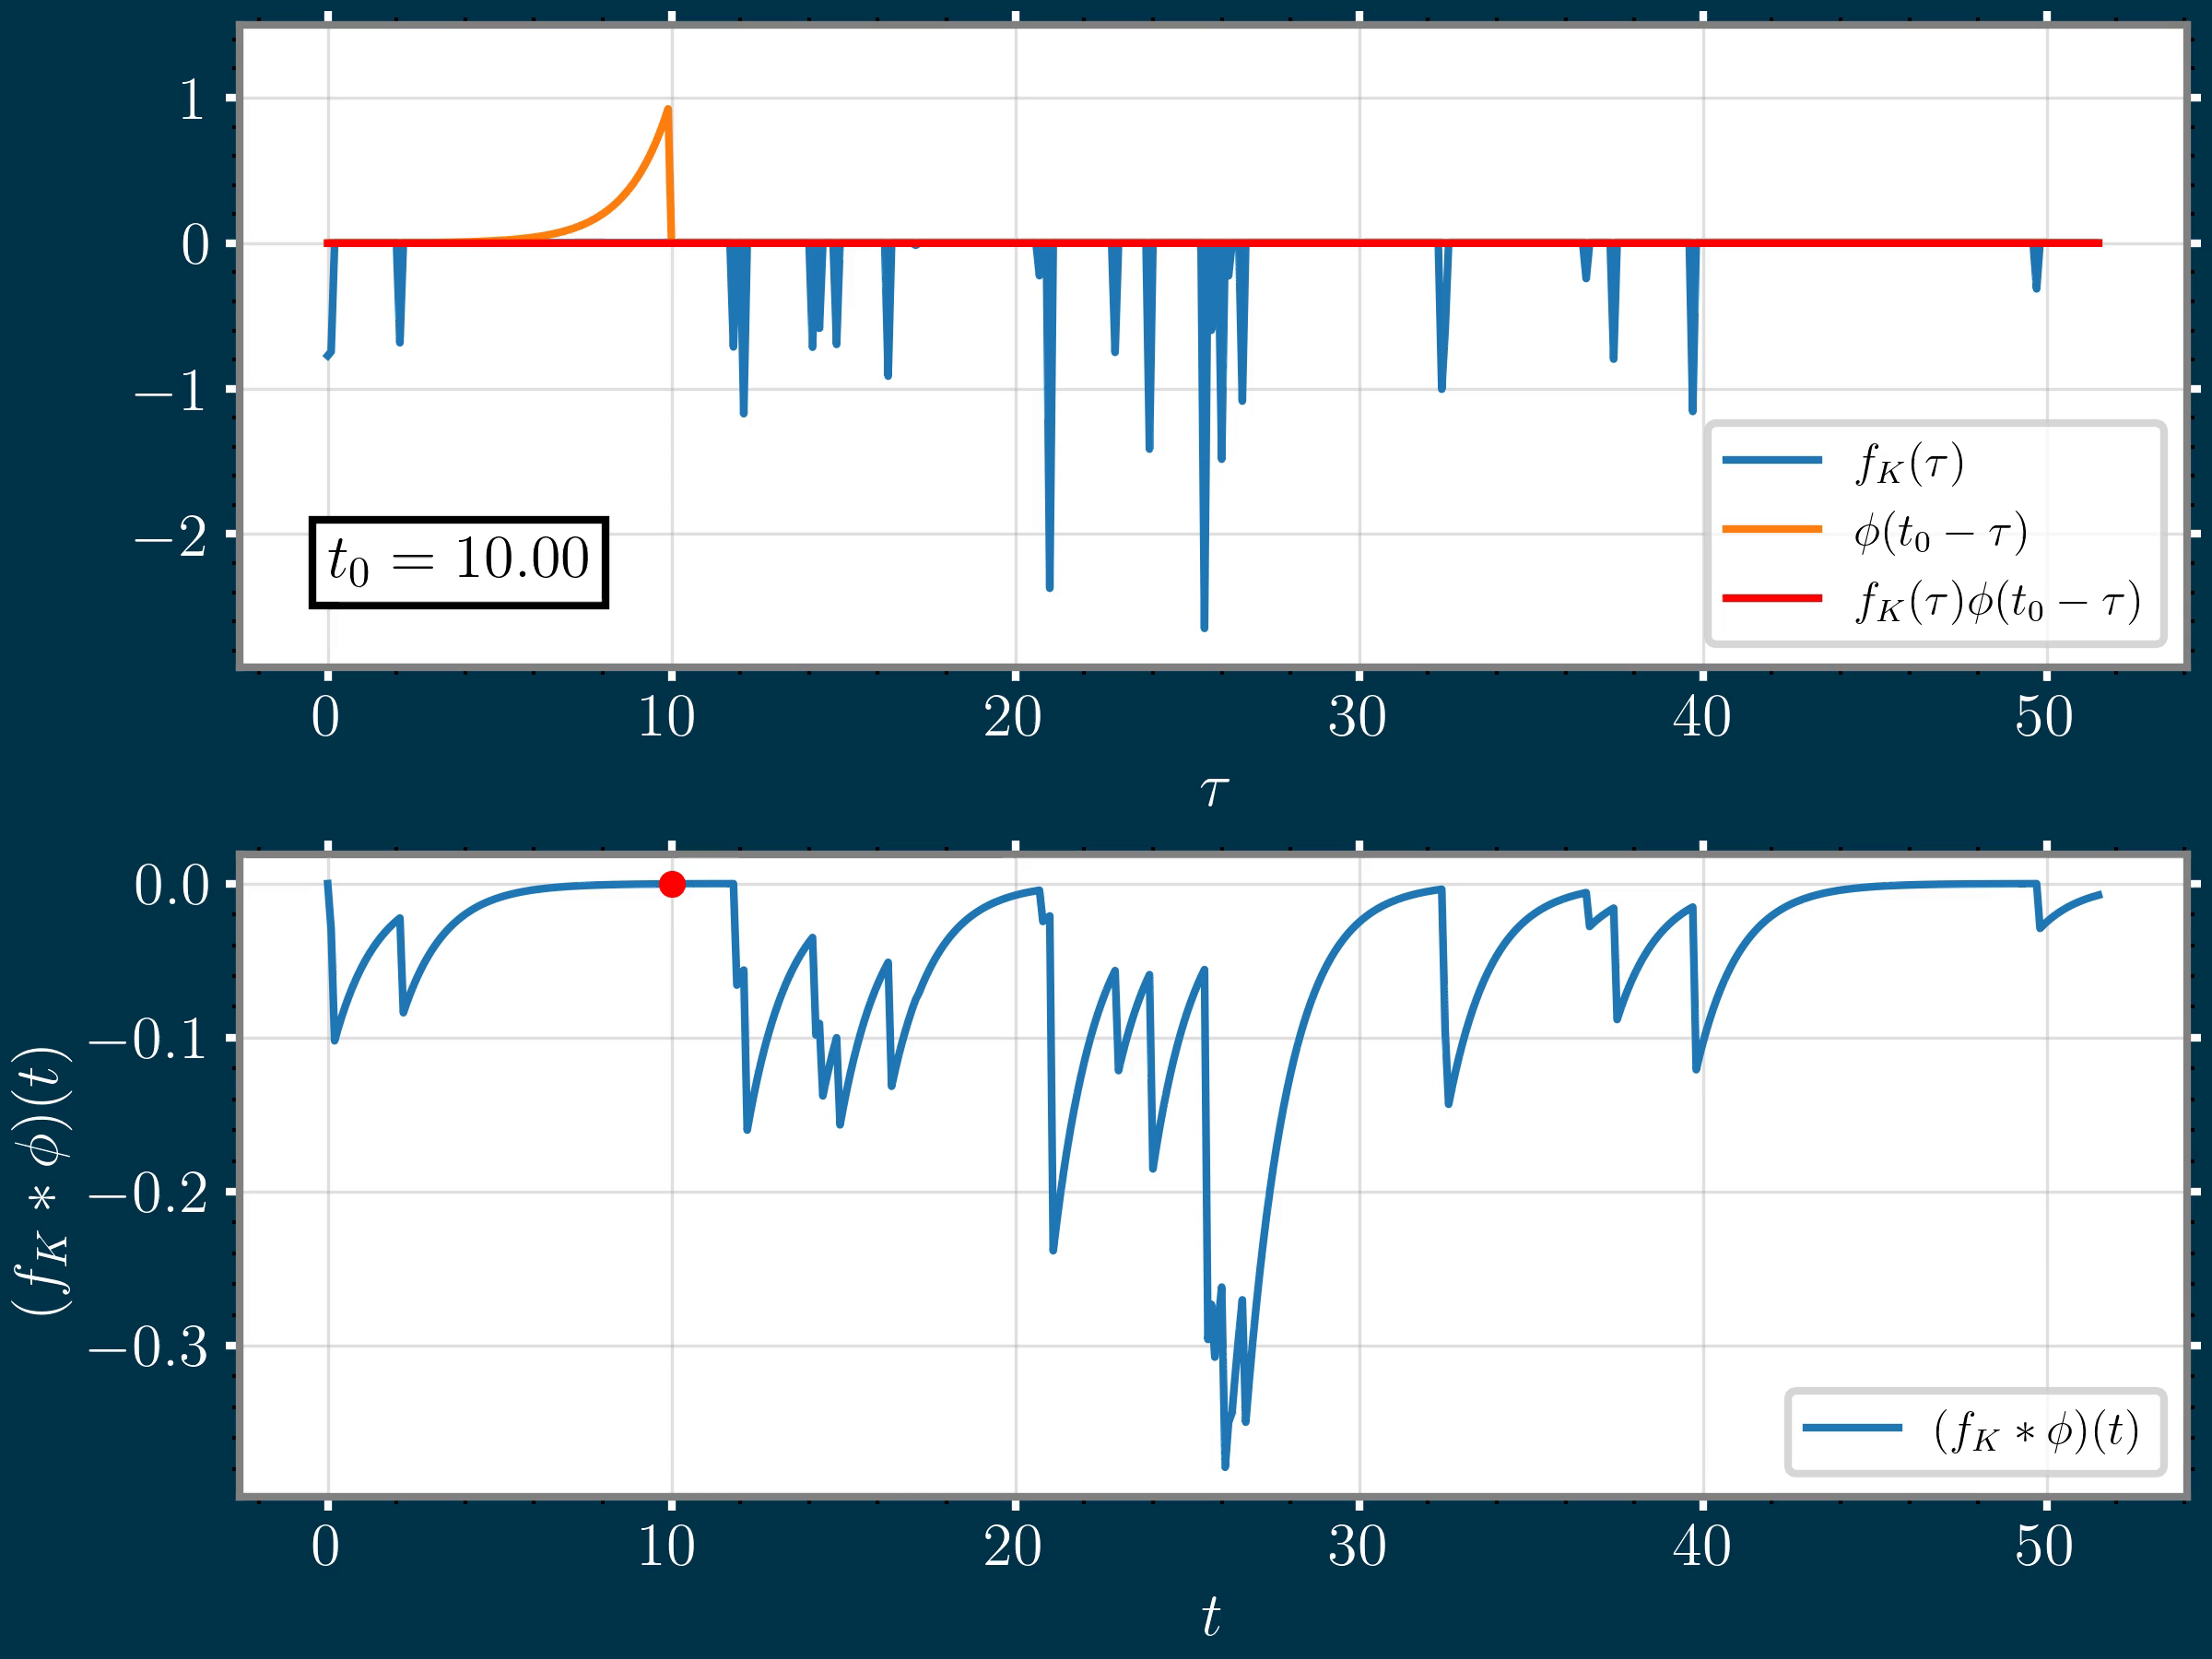
\includegraphics[width=.8\linewidth]{anim.png}
            \end{figure}
        \end{column}
    \end{columns}

    \note<+>{
        \begin{itemize}
            \item So let us look more closely at the FPP
            \item Superpos of individual volcanic events\ldots
        \end{itemize}
    }
    \note<+>{\ldots where each pulse has some amplitude \(A_k\)\ldots}
    \note<+>{\ldots they arrive according to a Poisson process at times \(t_k\)\ldots}
    \note<+>{\ldots and their duration is constant, given as \(\tau_\mathrm{d}\)}
    \note<+>{
        \begin{itemize}
            \item Can be written up as a convolution equation, where a common pulse
                shape is convolved with a forcing, which is also a sum of individual
                pulses, interpreted as volcanic eruptions
            \item We se in the animation how the convolution is done
            \item This assumes knowledge about the response function and the
                forcing, which gives you temperature as the output, so we need a method
                of turning it around
        \end{itemize}
    }

\end{frame}

% \begin{frame}{Simple raycasting animation}
%     \animategraphics[controls,loop,autoplay]{1}{conv-}{0}{16}
% \end{frame}

\begin{frame}{Filtered Poisson process --- Definition}

    The underlying phenemenological model:

    \begin{columns}
        \begin{column}{.51\linewidth}
            % \begin{equation}\label{eq:fpp_sum}
            %   % \alt<2>{T_K(t)}{\Phi_K(t)}=\sum_{k=1}^{\alt<2>{K}{K(T)}} A_k \phi\left(\frac{t-t_k}{\tau_\mathrm{d}}\right)
            %   T_K(t)=\sum_{k=1}^{K} A_k \phi\left(\frac{t-t_k}{\tau_\mathrm{d}}\right)
            % \end{equation}
            % \begin{equation*}
            %   \downarrow
            % \end{equation*}
            \begin{equation}\tag{\ref{eq:fpp_convolve}}
                % \alt<2>{T_K(t)}{\Phi_K(t)}=[\phi * f_K]\left(\frac{t}{\tau_\mathrm{d}}\right)
                T_K(t)=[\phi * f_K]\left(\frac{t}{\tau_\mathrm{d}}\right)
            \end{equation}
        \end{column}
        \begin{column}{.65\linewidth}
            \begin{center}
                % \animategraphics[autoplay,loop,width=.8\linewidth]{10}{gif/conv-}{0}{16}
                % 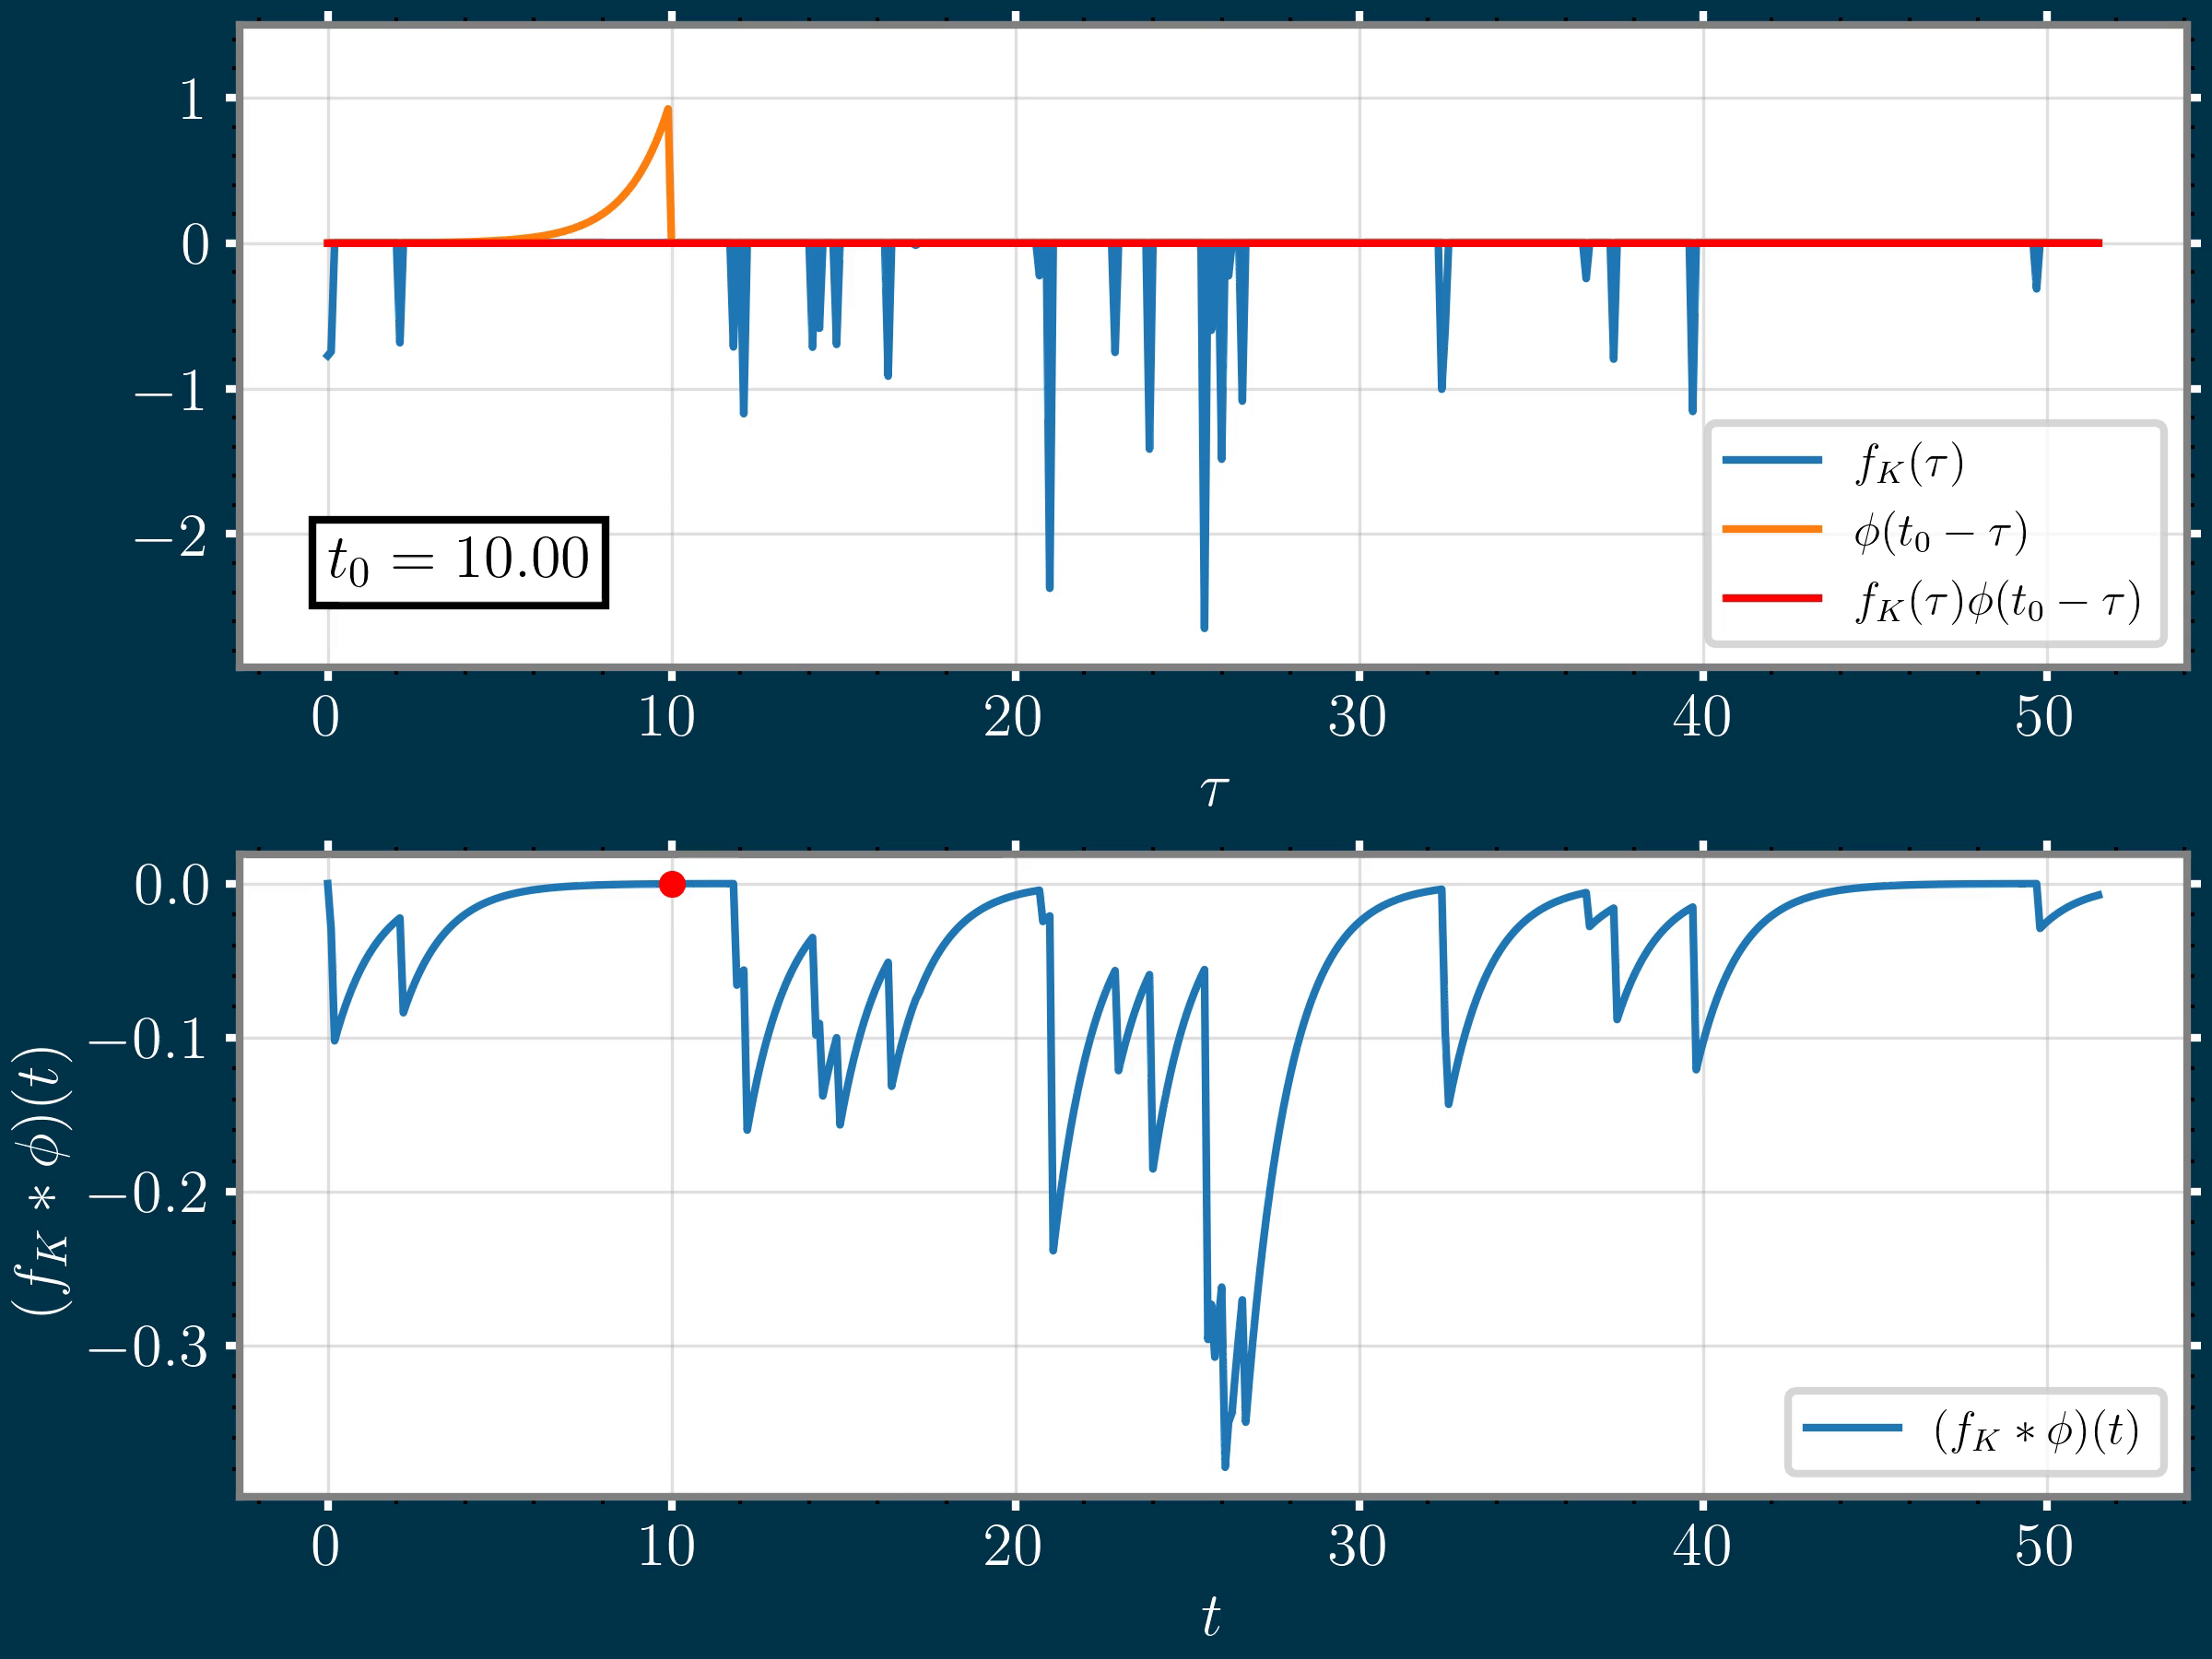
\includegraphics[width=.8\linewidth]{anim.png}
                \movie[
                height=.6\linewidth,
                width=.8\linewidth,
                autostart,
                loop
                ]{}{animation.mp4}
            \end{center}
        \end{column}
    \end{columns}

    \note<+>{
        \begin{itemize}
            \item So let us look more closely at the FPP
            \item Superpos of pulses with amplitudes \(A_k\), arrive according to a
                Poisson process at times \(t_k\) and their duration is constant:
                \(\tau_\mathrm{d}\)
            \item Can be written up as a convolution equation, where a common pulse
                shape is convolved with a forcing, which is also a sum of individual
                pulses, interpreted as volcanic eruptions
            \item We see in the animation how the convolution is done
            \item This assumes knowledge about the response function and the
                forcing, which gives you temperature as the output, so we need a method
                of turning it around
        \end{itemize}
    }

\end{frame}
% \begin{frame}
%   \frametitle{Filtered Poisson process --- Definition}

%   The underlying phenemenological model:

%   \begin{columns}
%     \begin{column}{.51\linewidth}
%       \begin{overprint}
%       \onslide<1>
%         \begin{equation}\label{eq:fpp_sum}
%           % \alt<2>{T_K(t)}{\Phi_K(t)}=\sum_{k=1}^{\alt<2>{K}{K(T)}} A_k \phi\left(\frac{t-t_k}{\tau_\mathrm{d}}\right)
%           \Phi_K(t)=\sum_{k=1}^{K(T)} A_k \phi\left(\frac{t-t_k}{\tau_\mathrm{d}}\right)
%         \end{equation}
%         \begin{equation*}
%           \downarrow
%         \end{equation*}
%         \begin{equation}\label{eq:fpp_convolve}
%           % \alt<2>{T_K(t)}{\Phi_K(t)}=[\phi * f_K]\left(\frac{t}{\tau_\mathrm{d}}\right)
%           \Phi_K(t)=[\phi * f_K]\left(\frac{t}{\tau_\mathrm{d}}\right)
%         \end{equation}
%       \onslide<2>
%       \begin{equation}\tag{\ref{eq:fpp_sum}}
%           % \alt<2>{T_K(t)}{\Phi_K(t)}=\sum_{k=1}^{\alt<2>{K}{K(T)}} A_k \phi\left(\frac{t-t_k}{\tau_\mathrm{d}}\right)
%           T_K(t)=\sum_{k=1}^{K} A_k \phi\left(\frac{t-t_k}{\tau_\mathrm{d}}\right)
%         \end{equation}
%         \begin{equation*}
%           \downarrow
%         \end{equation*}
%         \begin{equation}\tag{\ref{eq:fpp_convolve}}
%           % \alt<2>{T_K(t)}{\Phi_K(t)}=[\phi * f_K]\left(\frac{t}{\tau_\mathrm{d}}\right)
%           T_K(t)=[\phi * f_K]\left(\frac{t}{\tau_\mathrm{d}}\right)
%         \end{equation}
%       \end{overprint}
%     \end{column}
%     \begin{column}{.65\linewidth}
%       \begin{center}
%         \movie[
%           height=.6\linewidth,
%           width=.8\linewidth,
%           autostart,
%           loop
%           ]{}{animation.mp4}
%       \end{center}
%       % \begin{figure}
%       %   \centering
%       %   \animategraphics[autoplay,loop,width=\linewidth]{10}{../figures/deconvolution_anim/deconvolution_}{0}{52}
%       % \end{figure}
%     \end{column}
%   \end{columns}

% \end{frame}

% \begin{frame}
%   \frametitle{Filtered Poisson process --- Definition}

%   \begin{equation}\tag{\ref{eq:fpp_convolve}}
%     T_K(t)=[\phi * f_K]\left(\frac{t}{\tau_\mathrm{d}}\right)
%   \end{equation}

%   Given:
%   \begin{itemize}
%     \item \(\tau_\mathrm{d}\) is constant
%     \item \(f_K\) is a train of delta pulses:
%       \begin{equation}
%         f_K(t)=\sum_{k=1}^{K} A_k\delta\left(\frac{t-t_k}{\tau_\mathrm{d}}\right)
%       \end{equation}
%   \end{itemize}

% \end{frame}

\subsection{Deconvolution}

\begin{frame}{Richardson-Lucy deconvolution}

    An iterative process: \cite{Lucy1974,1972richardson,benvenuto2009}
    \begin{equation}\label{eq:deconvolution}
        \phi^{(n+1)}=\phi^{(n)} \frac{(T_K-\langle T_K\rangle)*\hat{f}_K+b}{\phi^{(n)}*f_K*\hat{f}_K+b}
    \end{equation}

    \note<+>{
        \begin{itemize}
            \item We write up a deconvolution equation, which is an iterative
                algorithm that can take forcing and temperature as the input, and out
                comes the response function
            \item The constant \(b\) regularises the process, ensuring positive
                definite response function
            \item Sajidah spent time discussing this algorithm and considerations
                that are important to account for
            \item It is not trivial, but we will simply apply it in this presentation
        \end{itemize}
    }

\end{frame}
